\chapter{System Design}
\label{ch:design}

This chapter describes how the pipeline is built: the architecture that turns
raw critical-care tables into a continuously updated, externally validated
sepsis-onset risk. The design links directly to the best practice established in
Chapter~\ref{ch:review}: leakage-safe temporal features, landmarking for
real-time risk, informative-missingness encoding, and a transportable
closed-form model.

\section{Overall Architecture}
The system is organised as a linear pipeline of numbered, single-purpose stages
grouped into three layers (\textbf{extract}, \textbf{model}, and
\textbf{evaluate}) as shown in Figure~\ref{image:sysArchitecture}. Each stage
reads the artefact written by the previous stage and writes its own, so any
stage can be re-run in isolation. A single configuration module is the sole
source of truth for file paths, clinical item identifiers, antibiotic name
lists, and Sepsis-3 thresholds.

\begin{figure}[h!]
    \centering
    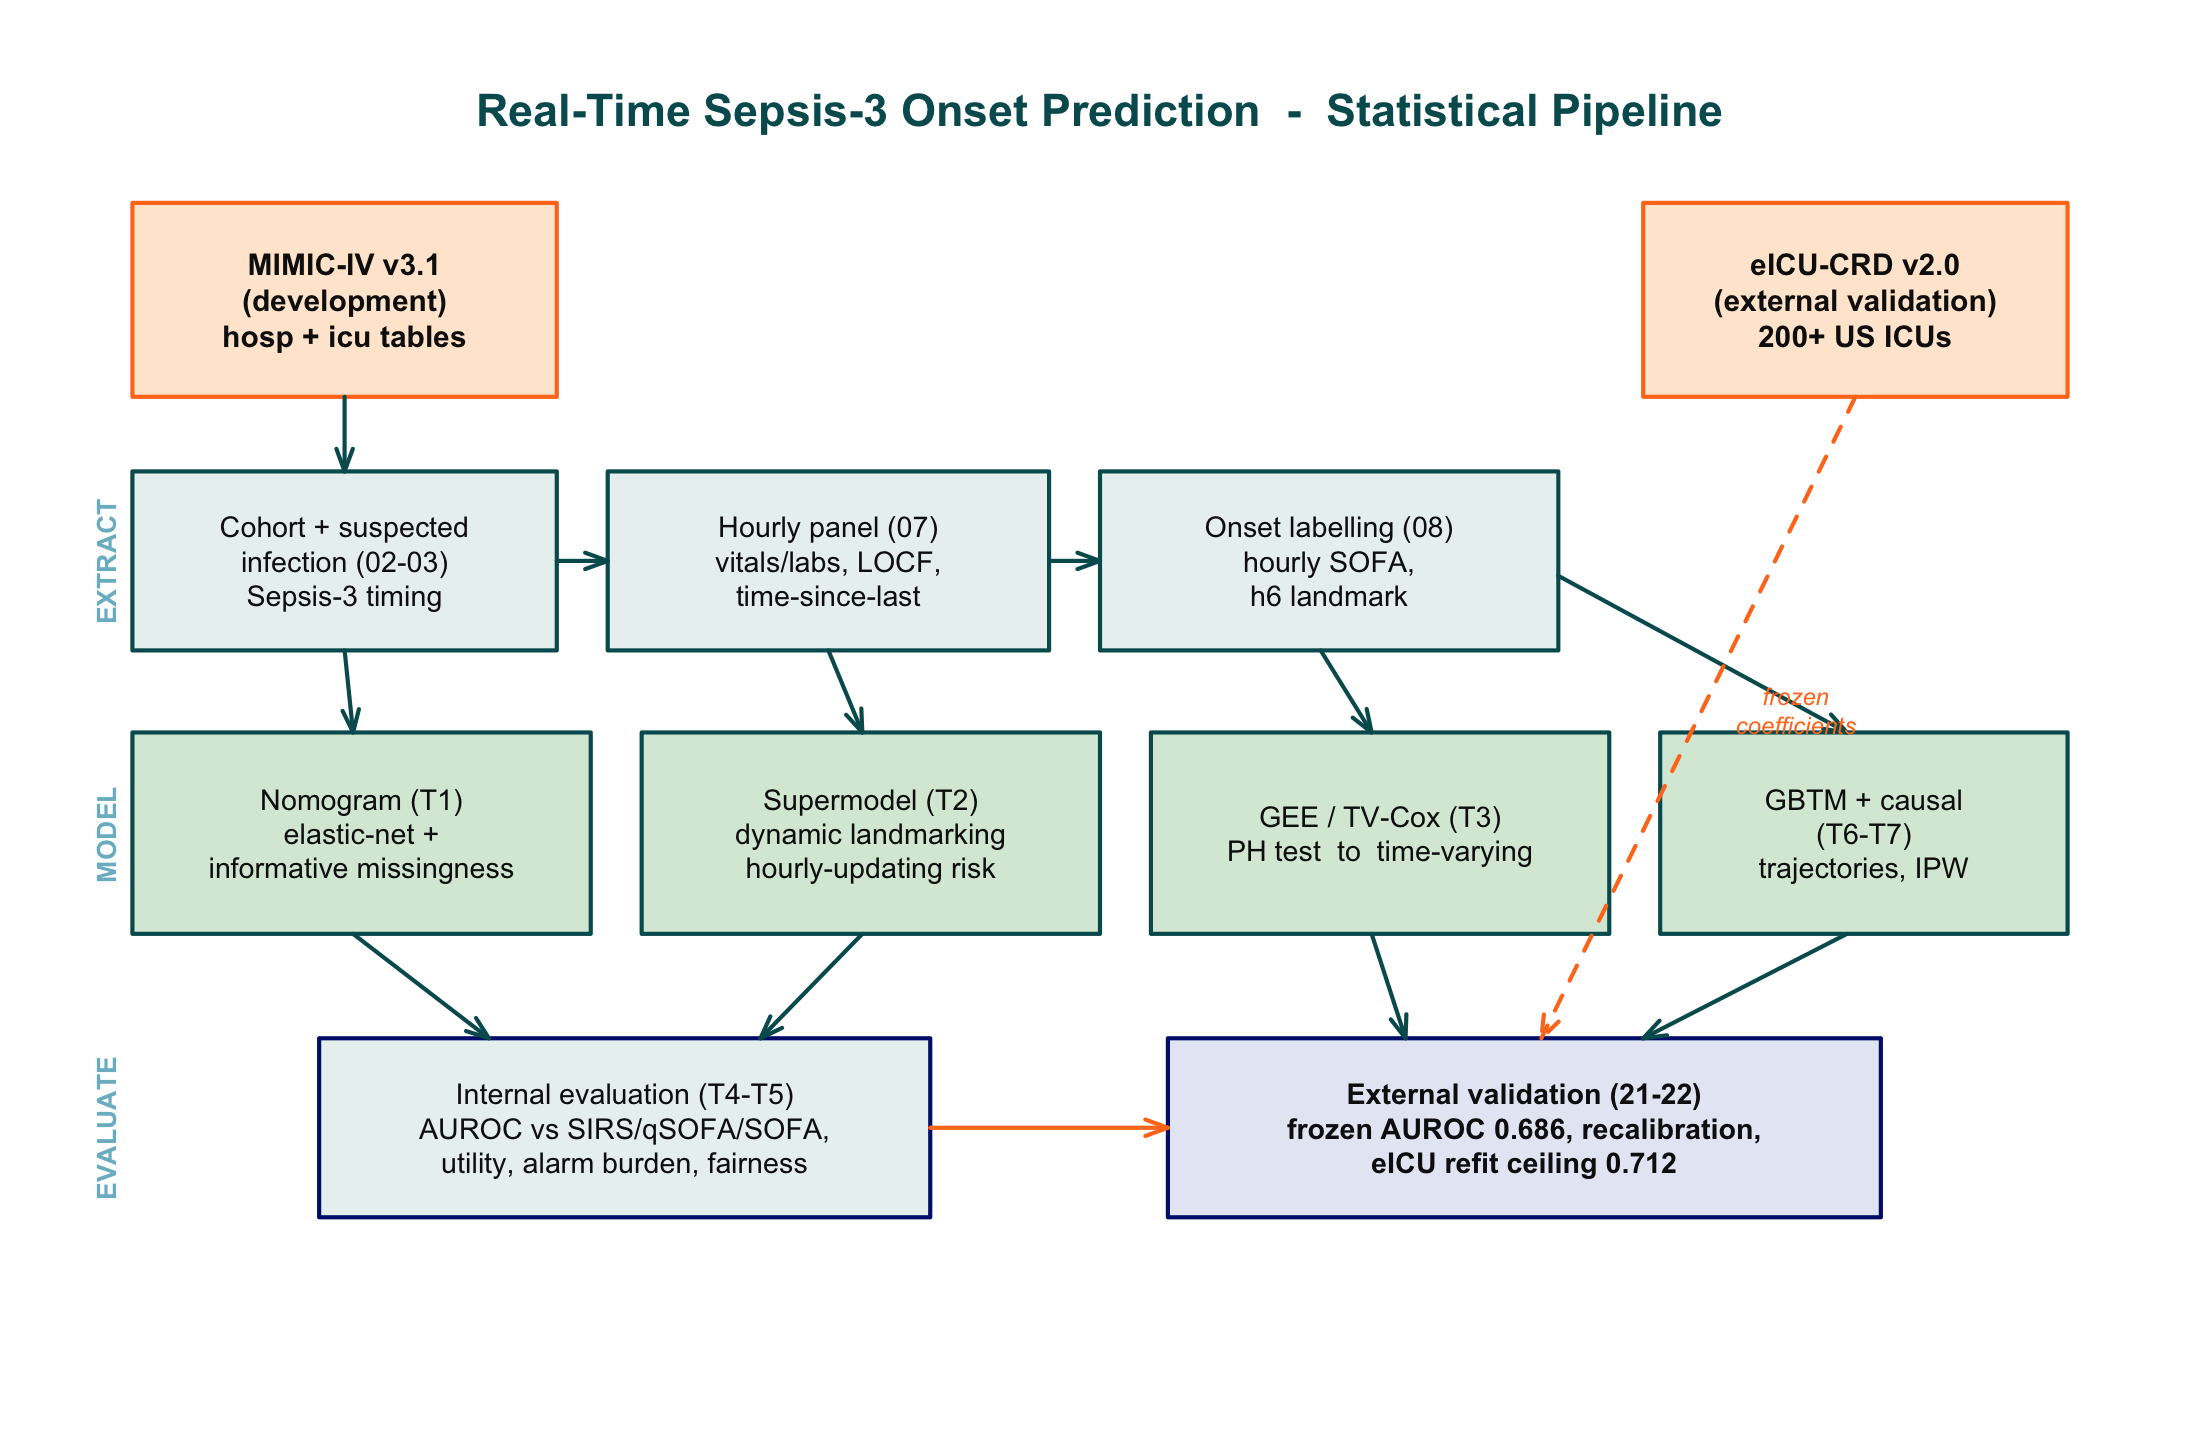
\includegraphics[width=0.98\textwidth]{images/architecture.png}
    \caption{System architecture: the extract, model, and evaluate layers. The
    development data (MIMIC-IV) flows through cohort construction, hourly panel
    assembly, and onset labelling into the statistical models; the frozen model
    coefficients are then transported to eICU-CRD for external validation.}
    \label{image:sysArchitecture}
\end{figure}

Figure~\ref{image:sysArchitecture} (referenced with
\textbf{\textbackslash{}ref\{image:sysArchitecture\}}) also records the key
external-validation result so that the architecture and its headline outcome can
be read together.

\section{Extract Layer}
The extract layer builds the analysis substrate. Cohort construction applies the
inclusion criteria (adults, first ICU stay, minimum length of stay) using only
the small administrative tables. Suspected-infection detection streams the
prescription and microbiology tables to pair antibiotics with cultures inside
the Sepsis-3 windows. The hourly-panel stage is the heaviest: it streams the
multi-gigabyte chart and lab tables in bounded-memory chunks and resamples every
stay onto an hourly grid, attaching for each core variable a forward-filled
value and a time-since-last-measured counter. The onset-labelling stage scores
hourly SOFA, locates the onset hour, and exports the hour-six landmark table
that the models consume.

\section{Model Layer}
The model layer implements the statistical tiers. The nomogram (Tier~1) is an
elastic-net penalised logistic regression at the hour-six landmark; its
informative-missingness design pairs each median-imputed laboratory value with a
binary ``was measured'' indicator. The supermodel (Tier~2) stacks the landmark
design across six landmark hours so that a single interpretable model emits
hourly-updating risk. Tier~3 addresses within-patient correlation using
generalised estimating equations with cluster-robust standard errors and fits a
time-varying Cox model after the proportional-hazards assumption is rejected.
Tiers~6 and~7 add group-based trajectory modelling and confounder-adjusted
causal estimates for early antibiotics. Every model is closed-form, so its
coefficients can be serialised and transported to a second database.

\section{Evaluate Layer}
The evaluate layer separates internal from external assessment. Internally
(Tiers~4--5), the models are scored for discrimination against the rule-based
baselines, for clinical utility and alarm burden, and for subgroup calibration
across sex and age. Externally, the hour-six landmark table is rebuilt on
eICU-CRD with the identical definitions, and the frozen MIMIC coefficients are
applied without refitting; a one-parameter recalibration and an eICU-native
refit are computed to separate miscalibration from any loss of discrimination.

\section{Implementation Notes}
Extraction and panel assembly are implemented in Python with pandas; the
statistical tiers and their reports are implemented in R. Intermediate artefacts
default to CSV for inspectability, with the two largest hourly panels stored as
columnar Parquet by necessity. All randomness uses a fixed seed, and the whole
sequence is reproducible from a single driver script that executes the stages in
order.
